\section{极限存在准则,两个重要极限}
\subsection{单调有界定理}

\begin{figure}[ht]
	\centering
	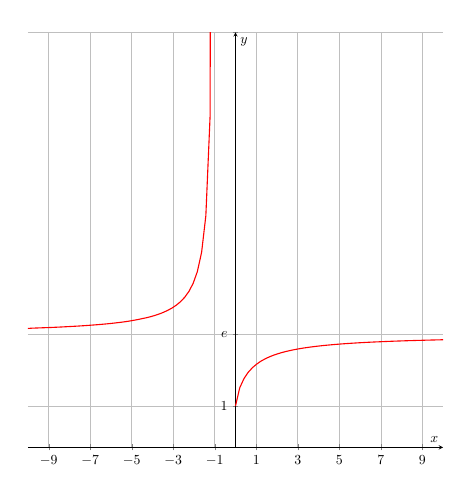
\begin{tikzpicture}[scale=.5]
	% Mathematica: Plot[{E,(1+1/x)^x},{x,-10,10},PlotRange->{0,10},AspectRatio->Automatic,PlotStyle->{{Dashed,Thin},Thin}]
		\begin{axis}[
			xmin=-10,xmax=10,ymin=0,ymax=10,
			grid=both,width=\textwidth,height=\textwidth,
			xlabel=$x$,
			ylabel=$y$,
			enlarge x limits=0.1,
			enlarge y limits=0.1,
			axis lines = middle,
			xtick={-9,-7,...,9},
			ytick={1,2.718,10},
			yticklabels={$1$,$e$},
		]
			\begin{scope}[samples=50,thick,red]
				\addplot[domain=-10:-0]{(1+1/x)^x};
				\addplot[domain=+0:+10]{(1+1/x)^x};
			\end{scope}
		\end{axis}
	\end{tikzpicture}
	\caption{函数\(y=\left(1+\tfrac{1}{x}\right)^x\)的图像}
	\label{figure:极限.函数(1+1/x)^x的图像}
\end{figure}

如\cref{figure:极限.函数(1+1/x)^x的图像} 所示,
我们可以画出函数\(y=\left(1+\frac1x\right)^x\ (x<-1 \lor x>0)\)的图像.
可见,直线\(y=e\)是函数\(y=\left(1+\frac1x\right)^x\)的图像的水平渐近线.
另外,易证\[
\lim_{x\to0^+} \left(1+\frac1x\right)^x = 1,
\qquad
\lim_{x\to1^-} \left(1+\frac1x\right)^x = +\infty.
\]


画出函数\(y=\left(1-\frac1x\right)^x\ (x<0 \lor x\geq1)\)的图像如\cref{figure:极限.函数(1-1/x)^x的图像}.
\begin{figure}[ht]
	\centering
	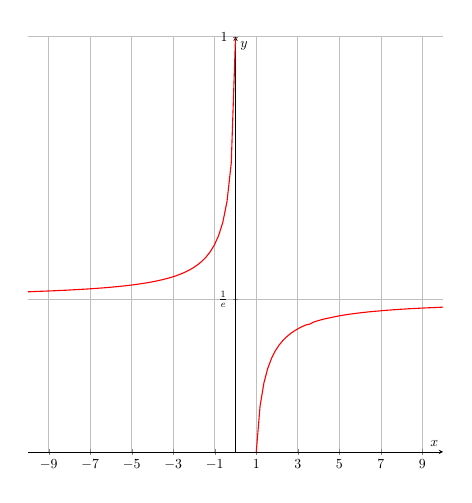
\begin{tikzpicture}[scale=.5]
		% Mathematica: Plot[{1/E, (1 - 1/x)^x}, {x, -10, 10}, PlotRange -> {0, 1}, PlotStyle -> {{Dashed, Thin}, Thin}]
		\begin{axis}[
			xmin=-10,xmax=10,
			ymin=0,ymax=1,
			grid=both,
			width=\textwidth,height=\textwidth,
			xlabel=$x$,
			ylabel=$y$,
			axis lines=middle,
			xtick={-9,-7,...,10},
			ytick={.3679,1},
			yticklabels={$\frac{1}{e}$,$1$},
		]
			\begin{scope}[samples=50,thick,red]
				\addplot[domain=-10:-0]{(1-1/x)^x};
				\addplot[domain=+1:+10]{(1-1/x)^x};
			\end{scope}
		\end{axis}
	\end{tikzpicture}
	\caption{函数\(y=\left(1-\tfrac{1}{x}\right)^x\)的图像}
	\label{figure:极限.函数(1-1/x)^x的图像}
\end{figure}
可见,直线\(y=\frac{1}{e}\)是函数\(y=\left(1-\frac1x\right)^x\)的图像的水平渐近线.
另外,易证\[
	\lim_{x\to0^-} \left(1-\frac1x\right)^x
	\xlongequal{t=-1/x} \lim_{t\to+\infty} \frac{1}{\sqrt[t]{1+t}}
	= 1.
\]
\end{example}

类似地,函数极限也有自己的柯西审敛原理.
